%% Towards a Cartography of Datacentering: A Multimodal Research Agenda
%% Target: Technological Forecasting and Social Change / Research Policy
%% Class: elsarticle

\documentclass[review,12pt,authoryear]{elsarticle}

\usepackage{hyperref}
\usepackage{amsmath}
\usepackage{graphicx}
\usepackage{booktabs}
\usepackage{array}
\usepackage{tabularx}
\usepackage{lineno}
\usepackage{microtype}
\usepackage{cleveref}

\modulolinenumbers[5]

\journal{Technological Forecasting and Social Change}

\bibliographystyle{elsarticle-harv}

\begin{document}

\begin{frontmatter}

\title{Towards a Cartography of Datacentering: A Multimodal Research Agenda}

\author[eur]{Babajide Owoyele\corref{cor1}}
\cortext[cor1]{Corresponding author}
\affiliation[eur]{organization={Erasmus University Rotterdam},
                  country={Netherlands}}

\begin{abstract}
Data centers are the material substrate of the digital economy — responsible for an estimated 400~TWh of electricity consumption annually and constituted by dense constellations of corporate, financial, civic, and governmental actors. Yet a bibliometric audit of 4,757 publications on data centers (OpenAlex, 2010--2025) reveals a striking blind spot: not one engages the Multi-Level Perspective, Technological Innovation Systems, Strategic Niche Management, or sociotechnical regimes frameworks that are standard equipment in innovation and sustainability transitions research. The literature fragments into three non-communicating silos — technical efficiency, environmental impact, and socio-political dynamics — none of which can account for the systemic, multi-actor character of the phenomena they study.

This paper proposes \textit{datacentering} as a conceptual reframing — a gerund that foregrounds the active, contested, ongoing process of assembling digital infrastructure rather than treating it as a stable technical object. Drawing on complex adaptive systems (CAS) thinking as a sensemaking lens, we develop a multimodal research agenda structured around the conceptual and structural dimensions of data center assemblages: how actors construct the imaginaries that make infrastructure legible or illegible, and how ownership hierarchies and actor constellations shape governance capacity. We propose four complementary methodological work packages — corporate and territorial text analysis, visual and satellite imagery analysis, ownership cartography, and contestation signal detection — and illustrate the analytical purchase of the framework through a comparison of Northern Virginia and Amsterdam.

We conclude that the complexity of data center assemblages as CAS-like phenomena demands not only multimodal methods but a collective, open approach to knowledge production. The paper is accompanied by an open research infrastructure — a community-maintained facility index, shared analytical pipelines, and open data — on the grounds that no single researcher or team can build this cartography alone.

\end{abstract}

\begin{keyword}
datacentering \sep digital infrastructure \sep complex adaptive systems \sep multimodal methodology \sep socio-material assemblage \sep financialisation \sep strategic invisibility \sep open research infrastructure
\end{keyword}

\end{frontmatter}

\linenumbers

%% Section 1 — Introduction
\section{Introduction}
\label{sec:introduction}

The infrastructure running the digital economy occupies a peculiar position in the scholarly literature: it is studied intensively in engineering and computer science, acknowledged briefly in environmental economics, contested occasionally in urban planning, but almost entirely absent from the fields — sustainability transitions, innovation systems, science and technology studies — that have developed the most sophisticated tools for understanding socio-material transformation. This paper begins from the premise that this absence is a problem for the field, not merely a gap for a research agenda to fill, and that correcting it requires both a conceptual reorientation and a methodological apparatus capable of reaching across the opacity that operators have deliberately constructed around their infrastructure.

Data centers now consume an estimated 400~TWh of electricity per year globally \citep{iea2024electricity}, a figure that makes them, collectively, among the fastest-growing industrial electricity users in OECD economies. They are physical: vast server halls, cooling towers that draw millions of litres of water daily, diesel generators staged for grid interruption, land parcels the size of small towns assembled quietly through option agreements and shell companies. They are contested: planning disputes, noise ordinances, water rights challenges, and community campaigns are a feature of markets from Loudoun County, Virginia to the outskirts of Dublin. They are governed — or systematically not governed — through structures that range from Real Estate Investment Trust (REIT) ownership dispersed across pension funds and retail investors to municipal moratoriums negotiated with named operators. And they are opaque by design: the term ``the cloud'' is not merely a marketing metaphor but an ideological instrument that naturalises infrastructure, makes it seem weightless and placeless, and thereby insulates it from the territorial accountability that its material footprint would otherwise attract.

%% Box 1 — Megaprojects capex comparison and its limits

\begin{fullwidth}
\begin{tcolorbox}[datacenterbox,
  title={Box 1\enspace Data centers as a megaproject? Scale, comparability, and the limits of the analogy}]

\begin{minipage}[t]{\linewidth}
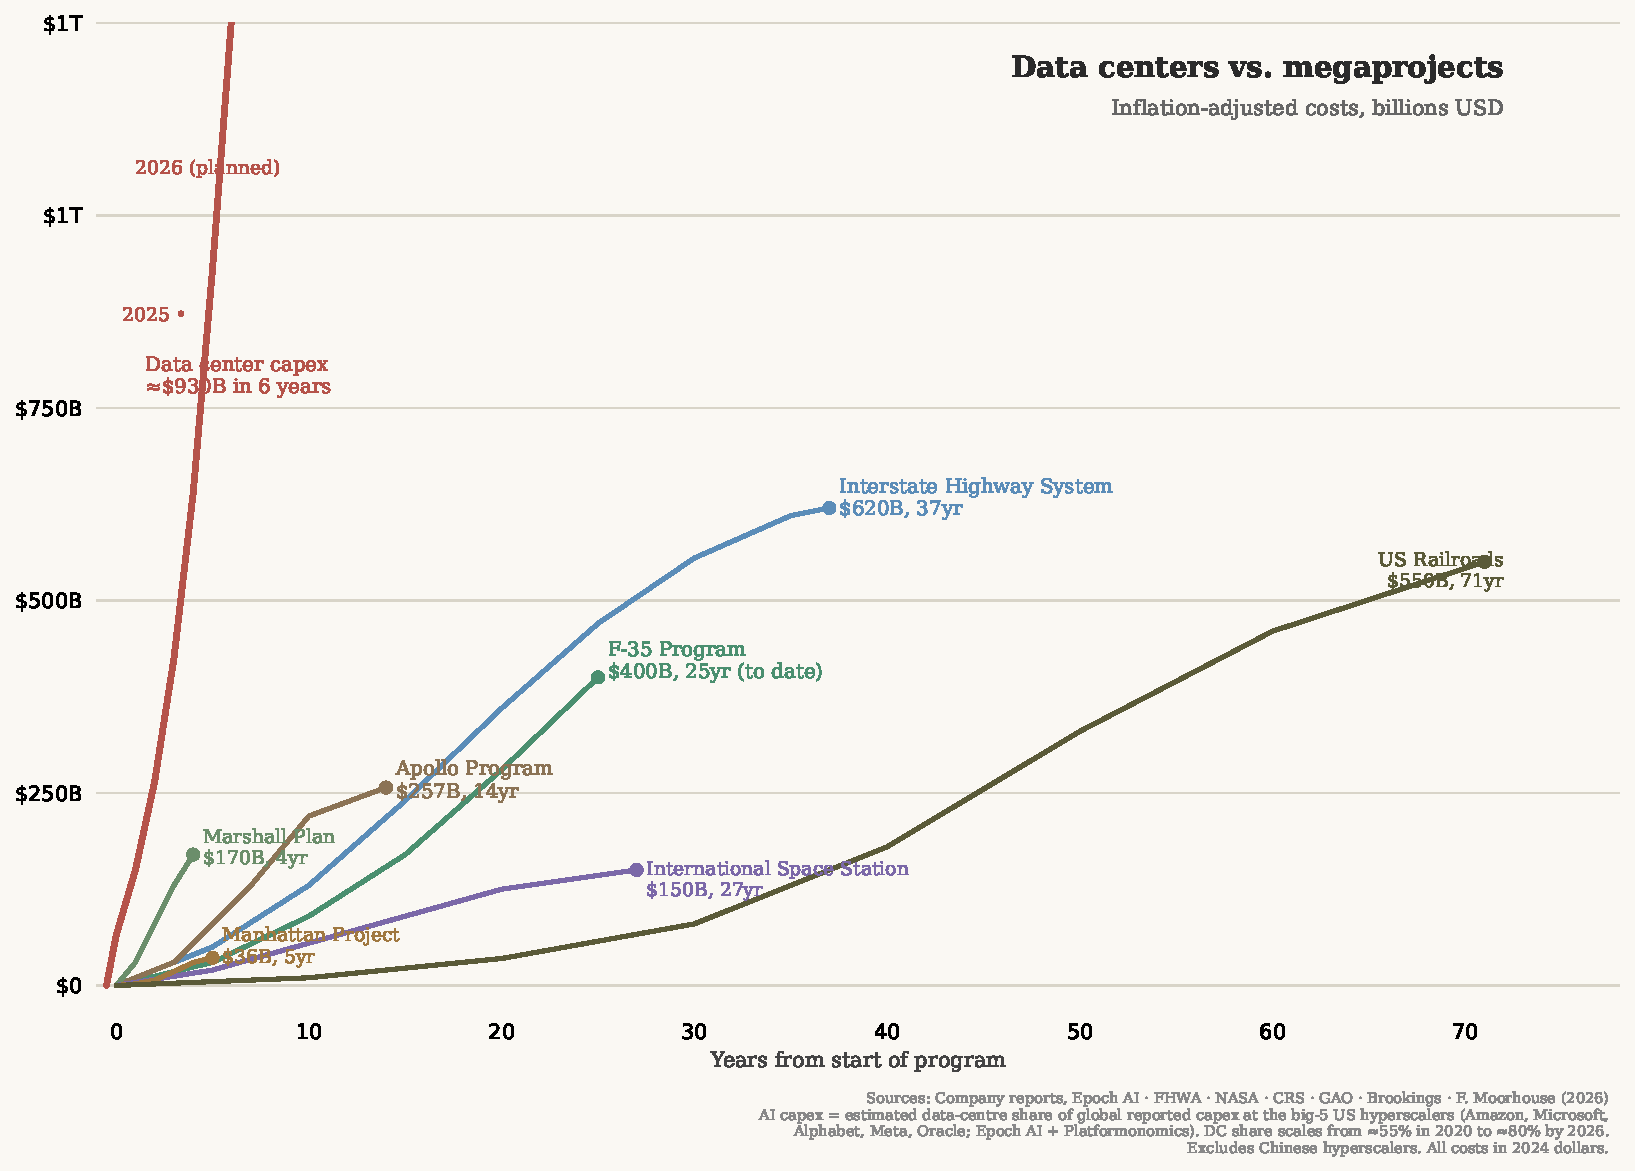
\includegraphics[width=\linewidth]{figures/megaprojects_capex}
\vspace{0.3em}
{\footnotesize\textit{Figure.} Cumulative data center capex (2019--2025, projected 2026) against
historical megaprojects, inflation-adjusted 2024 USD. Data: Epoch AI / Platformonomics;
FHWA; NASA; CRS; GAO; Brookings. Chart style after \citet{moorhouse2026megaprojects}.
All costs in 2024 dollars; Chinese hyperscalers excluded.}
\end{minipage}

\smallskip\noindent\rule{\linewidth}{0.3pt}\smallskip

\noindent\textbf{Why the comparison is powerful — and why it is also misleading.}\enspace
The chart circulates widely as evidence that data center investment has become the
defining infrastructure programme of the present moment, surpassing in speed and
aggregate cost anything the public sector has attempted since the Interstate Highway
System. As a rhetorical device it works: the visual comparison compresses the argument
into a single image.

As an analytical claim, however, the comparison conflates incommensurable categories.
\textit{First}, private recurring capital expenditure — distributed across thousands of
facilities, operators, and jurisdictions, repaid through commercial returns — is
structurally different from one-off public programmes underwritten by sovereign credit
and motivated by collective goods. The Apollo Programme produced the Moon landing and
was then wound down; data center capex is an indefinitely renewing operational
commitment whose cumulative figure grows by definition every year.
\textit{Second}, the comparison exploits the asymmetry of cumulation: summing six years
of annual private capex and setting it against the total lifetime cost of a 37-year
programme makes the former appear commensurately large, but the correct comparison is
the annual \textit{rate} of investment — at which point the Interstate Highway System
absorbed a larger share of US GDP for longer than the current data center build-out.
\textit{Third}, the data center capex figure rests on an opaque imputation methodology
(a DC share of hyperscaler capex scaling from $\approx$55\% to $\approx$80% across
the period) that is not independently verifiable and excludes Chinese hyperscalers
whose inclusion would substantially alter the comparison.
\textit{Fourth}, the selection of comparators does rhetorical work: there is no
equivalent chart for telecoms network buildout (1990--2000), rural electrification
(1935--1950), or the transatlantic cable system — all of which would likely produce
similar or larger figures on the same axes.

The chart is cited here not as authoritative evidence of scale but as a data point
about the \textit{genre of claim} being made about data centers in public discourse.
The fact that this particular comparison circulates as widely as it does — through
Epoch AI reports, policy briefs, and social media — is itself a finding: it indicates
that the governance and accountability frameworks for data center infrastructure are
being formed in an environment where the dominant reference points are wartime
mobilisation and Cold War programmes, not the regulatory regimes developed for
utilities, telecommunications, or land-use planning. The analogy shapes what
interventions appear plausible.

\end{tcolorbox}
\end{fullwidth}


A bibliometric audit of 4,757 publications with ``data center'' in the title on OpenAlex (2010--2025) makes the disciplinary gap visible in quantitative terms. The literature has grown by 372\% over fifteen years and organised itself into three structurally disconnected silos: technical efficiency (approximately 279 papers focused on cooling, power management, and hardware optimisation), environmental impact (approximately 114 papers, primarily on carbon footprint and energy sourcing), and socio-political dynamics (approximately 15 papers, including the rich ethnographic literature of \citet{vonderau2019storing} and \citet{holt2015vonderau}). Zero papers in this corpus engage the Multi-Level Perspective, Technological Innovation Systems, Strategic Niche Management, or sociotechnical regimes — the frameworks through which innovation scholars routinely analyse infrastructure transitions of comparable scale and consequence. The ethnographic work that does exist is invisible to this audience, and the innovation literature has not noticed the gap (\Cref{tab:silos}).

%% Inline tables — called from within body sections

%% ============================================================
%% Table 1 — Literature silos (called from sec:introduction)
%% ============================================================

\begin{table}[ht]
\centering
\caption{Three disconnected silos in the data center literature (OpenAlex, 2010--2025, $n = 4{,}757$).
         Representative works indicate the most-cited papers within each silo.
         The zero-paper row for innovation studies is the starting point of this research agenda.}
\label{tab:silos}
\setlength{\tabcolsep}{6pt}
\renewcommand{\arraystretch}{1.35}
\begin{tabularx}{\textwidth}{>{\bfseries}lXrX}
\toprule
\rowcolor{dcblue}
\textcolor{white}{\textbf{Silo}} &
\textcolor{white}{\textbf{Core focus}} &
\textcolor{white}{\textbf{$\approx n$}} &
\textcolor{white}{\textbf{Representative works}} \\
\midrule
Technical efficiency &
  Cooling infrastructure, power usage effectiveness (PUE), hardware lifecycle, workload scheduling, heat reuse &
  279 &
  \citet{dayarathna2015data}; Koomey (2011); \citet{masanet2020recalibrating} \\
\addlinespace[2pt]
\rowcolor{dcgray}
Environmental impact &
  Carbon footprint, scope 2 emissions, renewable energy PPAs, water withdrawal intensity &
  114 &
  \citet{iea2024electricity}; Jones (2018); Mytton \& Ashtine (2022) \\
\addlinespace[2pt]
Socio-political &
  Ethnography of infrastructure, planning disputes, cultural politics, local community impact &
  15 &
  \citet{blum2012tubes}; \citet{holt2015vonderau}; \citet{vonderau2019storing} \\
\addlinespace[4pt]
\rowcolor{dcaccent!12}
\textit{Innovation studies} &
  \textit{MLP, TIS, SNM, sociotechnical regimes, transition governance} &
  \textcolor{dcaccent}{\textbf{0}} &
  \textit{--- this paper ---} \\
\bottomrule
\end{tabularx}
\end{table}

%% ============================================================
%% Table 2 — Work packages (called from sec:introduction or sec:conceptual)
%% ============================================================

\begin{table}[ht]
\centering
\caption{The four work packages: CAS dimensions, data modalities, analytical outputs, and current implementation status.
         ``Seed'' denotes a pilot run against the three-operator facility index; ``design'' denotes a work package
         whose pipeline architecture is specified but not yet implemented.}
\label{tab:wps}
\setlength{\tabcolsep}{5.5pt}
\renewcommand{\arraystretch}{1.35}
\begin{tabularx}{\textwidth}{c>{\bfseries}lllXl}
\toprule
\rowcolor{dcblue}
\textcolor{white}{\textbf{WP}} &
\textcolor{white}{\textbf{CAS Dimension}} &
\textcolor{white}{\textbf{Primary method}} &
\textcolor{white}{\textbf{Data sources}} &
\textcolor{white}{\textbf{Key analytical output}} &
\textcolor{white}{\textbf{Status}} \\
\midrule
\textbf{1} & Conceptual &
  NLP / keyword scoring &
  Corporate websites; city Wikipedia &
  Environmental Claim Index (ECI); imaginary divergence score per operator--city pair &
  Seed run \\
\addlinespace[2pt]
\rowcolor{dcgray}
\textbf{2} & Conceptual &
  Computer vision (CLIP) &
  Sentinel-2 satellite imagery; corporate photography &
  Visual abstraction score; satellite--corporate imagery divergence &
  Design \\
\addlinespace[2pt]
\textbf{3} & Structural &
  Network analysis; spatial graph &
  OpenCorporates; REIT filings; Overture Maps (city2graph) &
  Ownership network + actor typology; urban embeddedness graph &
  Seed run \\
\addlinespace[2pt]
\rowcolor{dcgray}
\textbf{4} & Structural + Temporal &
  Topic modelling (BERTopic); event detection &
  News archives (GDELT/NewsAPI); planning records; social media &
  Signal-to-response lag; comparative contestation trajectory &
  Design \\
\bottomrule
\end{tabularx}
\end{table}

%% ============================================================
%% Table 3 — Virginia vs Amsterdam comparison
%% (called from sec:case)
%% ============================================================

\begin{table}[ht]
\centering
\caption{Comparative dimensions: Northern Virginia (Loudoun County) and Amsterdam.
         Both markets exhibit high community contestation intensity.
         The decisive variable differentiating regime responses is not signal strength
         but the structural architecture of the receiving system.
         ECI figures from WP1 seed run (April 2026); urban embeddedness from WP3 seed run (April 2026).}
\label{tab:comparison}
\setlength{\tabcolsep}{6pt}
\renewcommand{\arraystretch}{1.4}
\begin{tabularx}{\textwidth}{>{\bfseries\small}lXX}
\toprule
\rowcolor{dcblue}
\textcolor{white}{\textbf{Dimension}} &
\textcolor{white}{\textbf{Northern Virginia (Loudoun County)}} &
\textcolor{white}{\textbf{Amsterdam}} \\
\midrule
Operator type &
  Hyperscale (AWS, Microsoft, Google, Meta) + colocation (Equinix, Digital Realty, CyrusOne) &
  Hyperscale + colocation (Equinix AMS campus) + cooperative exchange (AMS-IX) \\
\addlinespace[2pt]
\rowcolor{dcgray}
Ownership structure &
  REIT-dominated; beneficial ownership dispersed across global pension funds and retail investors &
  Mixed; operator-owned campuses, cooperative exchange, concentrated sovereign wealth fund positions \\
\addlinespace[2pt]
Governance counterparty &
  None identifiable; operating entity legally separated from asset-owning REIT &
  Municipality (Amsterdam) with legal planning competence; named operator counterparties \\
\addlinespace[2pt]
\rowcolor{dcgray}
Urban embeddedness (2~km) &
  36 power-infra nodes; \textbf{1} residential zone; \textbf{0} adjacency edges~--- exurban spatial segregation &
  2 power nodes; \textbf{61} residential zones; \textbf{16} adjacency edges~--- embedded in urban fabric \\
\addlinespace[2pt]
Territorial imaginary &
  Opportunity framing; placeless; ECI divergence \textbf{165.7} (corp 167.1 vs.\ wiki 1.4) &
  Contested, partially negotiated; lower ECI divergence; regulatory vocabulary absorbed \\
\addlinespace[2pt]
\rowcolor{dcgray}
Visual regime &
  High abstraction; hyperscale anonymity; near-zero facility-level disclosure &
  Lower abstraction; higher regulatory disclosure requirements; urban-context imagery \\
\addlinespace[2pt]
Contestation intensity &
  High; community campaigns, planning hearing backlogs, state-level water studies &
  High; sustained municipal and civic mobilisation, media coverage, moratorium petitions \\
\addlinespace[2pt]
\rowcolor{dcgray}
Regime response &
  None; no moratorium; operator-accommodating state permitting environment &
  Moratorium declared 2019; enforced 2019--2022; lifted under differentiated energy/water criteria \\
\addlinespace[4pt]
\rowcolor{dclightyellow}
\multicolumn{1}{>{\bfseries\small\color{dcaccent}}l}{Explanatory variable} &
  \textcolor{dcaccent}{Dispersed ownership and absent governance counterparty insulate regime from community pressure} &
  \textcolor{dcblue}{Concentrated, accountable ownership + empowered municipal authority enable binding negotiation} \\
\bottomrule
\end{tabularx}
\end{table}


This paper makes three contributions in response. First, it proposes \textit{datacentering} as a conceptual reframing — a gerund that foregrounds the active, contested, ongoing process of assembling digital infrastructure over time, rather than treating data centers as fixed technical objects amenable to efficiency optimisation. Second, it develops a multimodal research agenda structured around the conceptual and structural dimensions of these assemblages, drawing on complex adaptive systems (CAS) thinking \citep{phillips2019complex} as a sensemaking lens for understanding phenomena that are constituted by multi-actor constellations — corporations, financial investors, planning authorities, municipal governments, communities, and nonhuman actors including power grids, aquifers, and fibre networks — whose interactions produce emergent, nonlinear outcomes no single actor controls. Third, it argues that the CAS-like character of these phenomena is itself the reason why no single researcher or team can build the cartography required: the geography is too large, the data too distributed, and the opacity too deliberate. We therefore accompany this paper with an open research infrastructure — a community-maintained facility index, shared analytical pipelines, and open data — as a theoretically motivated response to the complexity of the object, and as an invitation to collective knowledge production.

The paper proceeds as follows. \Cref{sec:background} reviews the relevant literature and introduces the concept of datacentering and the CAS sensemaking lens. \Cref{sec:conceptual} develops the conceptual dimension of the research agenda, addressing how actors construct the imaginaries and territorial claims that make data center infrastructure legible or illegible. \Cref{sec:structural} addresses the structural dimension, mapping the ownership hierarchies and actor constellations — including the urban and municipal actors that the city2graph framework \citep{city2graph} makes tractable — through which governance capacity (or its absence) is constituted. \Cref{sec:temporal} addresses the temporal dimension, examining how contestation signals unfold over time and what determines whether regime actors respond. \Cref{sec:case} illustrates the framework through a comparison of Northern Virginia and Amsterdam, two markets with equivalent contestation intensity but structurally different governance responses. \Cref{sec:discussion} draws out the theoretical implications and positions the open cartography as a research programme. \Cref{sec:conclusion} closes with the invitation to build it together.

%% Section 2 — Conceptual Background
\section{Conceptual Background}
\label{sec:background}

\subsection{The literature and its limits}

The existing literature on data centers is, in aggregate, large and growing. But its organisation into disconnected silos is not incidental to the phenomena it studies — it is a product of the disciplinary assumptions each silo imports. The technical efficiency literature treats data centers as engineering optimisation problems: cooling infrastructure, power usage effectiveness ratios, hardware lifecycle management. The environmental impact literature treats them as emissions sources to be measured and, where possible, reduced. The socio-political literature — thinner, more dispersed, and largely invisible to the other two — treats them as sites of ethnographic interest, following \citet{blum2012tubes}, \citet{holt2015vonderau}, and \citet{vonderau2019storing} in attending to the material, political, and cultural dimensions of infrastructure that the engineering literature abstracts away.

None of these literatures possesses the conceptual tools to account for data centers as a \textit{systemic} phenomenon: an infrastructure regime being constituted through the ongoing interactions of heterogeneous actors across multiple scales, involving feedback loops between technological change, investment structures, planning systems, community mobilisation, and regulatory response. This is precisely the terrain for which the Multi-Level Perspective \citep{geels2002technological}, Technological Innovation Systems, and sociotechnical regime analysis were developed — and it is, as the bibliometric audit establishes, terrain they have not yet entered.

\subsection{Datacentering as a concept}

We propose \textit{datacentering} as a conceptual reframing adequate to this terrain. The choice of a gerund is deliberate. Where ``data center'' names a technical object with fixed properties, ``datacentering'' names a \textit{process}: the ongoing, contested, socio-material practice of assembling, operating, expanding, and reproducing digital infrastructure in particular places, by particular actors, for particular purposes, under particular conditions of governance and resistance. The concept draws on two theoretical lineages.

The first is \citeauthor{orlikowski2007sociomaterial}'s \citeyear{orlikowski2007sociomaterial} account of sociomaterial practice: the claim that technology and social practice are constitutively entangled rather than separately analysable. A data center is not a technical substrate onto which social processes are then layered; the servers, the cooling towers, the power contracts, the planning permissions, the community objections, and the financial instruments are all co-constitutive elements of the same socio-material assemblage. To study the assemblage, one must be able to reach all its elements — hence the multimodal agenda this paper develops.

The second lineage is the sociology of sociotechnical imaginaries \citep{jasanoff2015dreamscapes}: the claim that the representations through which actors understand and communicate about technology are not mere descriptions of material facts but co-producers of those facts. ``The cloud'' is the paradigm case. It is an imaginary that naturalises infrastructure, decouples computation from territory, and positions data center campuses as nodes in a universal technical commons rather than as large-scale industrial land uses embedded in specific watersheds, power grids, and communities. The imaginary does not merely describe the infrastructure; it shapes how planning systems respond to it, how investors price it, how communities mobilise against it, and how operators justify their presence to municipal authorities. Datacentering is, in part, the continuous work of maintaining and contesting this imaginary.

\subsection{Complex adaptive systems as a sensemaking lens}

We draw on complex adaptive systems (CAS) thinking not as a formal operationalised framework but as a sensemaking lens: a way of apprehending the systemic character of the phenomena before deciding how to study them. \citet{phillips2019complex} provide the most directly applicable treatment, proposing a CAS-based methodology for ecosystem research organised around three dimensions: \textit{conceptual} (boundaries, perspectives, and imaginaries: how we think about the system), \textit{structural} (hierarchy, relationships, and actor constellations: what we know about the system), and \textit{temporal} (dynamics and co-evolution: how the system changes over time).

Applied to datacentering, the CAS lens immediately surfaces features — illustrated in \Cref{fig:constellation} — that that the existing literature misses. The actor constellation is genuinely heterogeneous: hyperscale operators, colocation providers, REIT asset managers, pension fund investors, cloud computing tenants, municipal authorities, planning inspectors, community campaign groups, environmental regulators, energy grid operators, and water utilities are all constitutive actors in the assemblage — not merely context for it. Their interactions are nonlinear: the same intensity of community contestation produces a planning moratorium in Amsterdam and no discernible governance response in Northern Virginia, a difference not explicable by the strength of the signal but by the structural properties of the system receiving it. And the outcomes are emergent: no single actor in the Loudoun County data center market planned for it to become the highest-concentration cluster in the world; that outcome is the emergent product of thousands of individual location, investment, and planning decisions interacting under conditions no single actor controlled.

\begin{fullwidth}
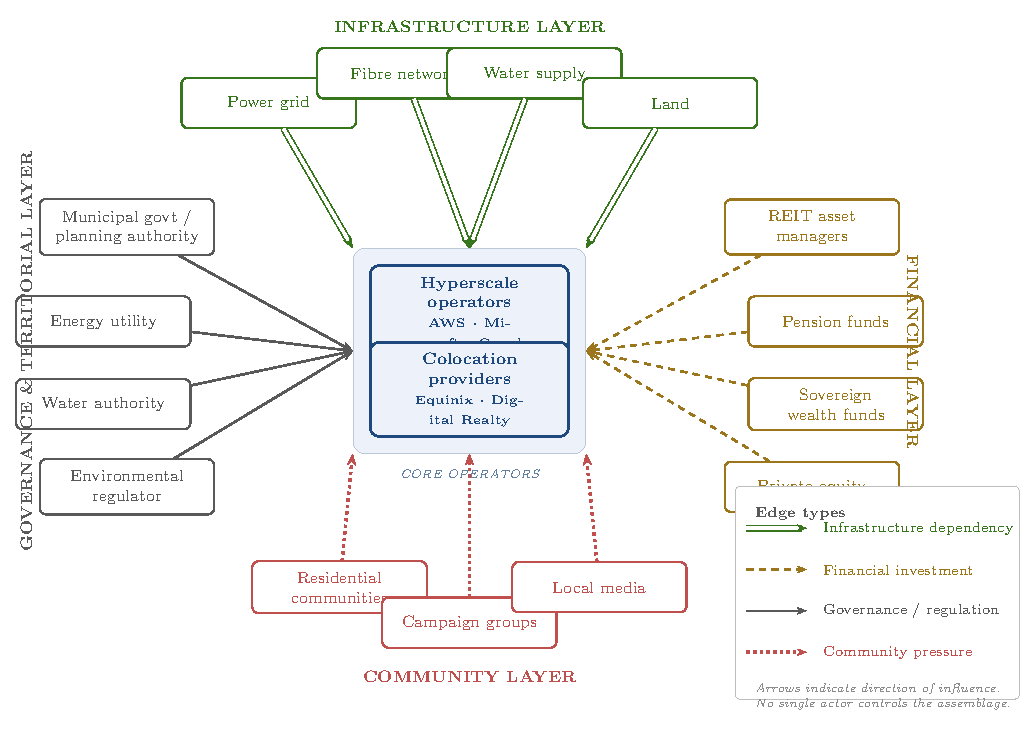
\includegraphics[width=\linewidth]{figures/actor-constellation}
\vspace{0.4em}
\captionof{figure}{The multi-actor constellation of a data center assemblage. No single actor controls the system; outcomes are emergent products of interactions across corporate, financial, governance, community, and infrastructure layers.\label{fig:constellation}}
\end{fullwidth}

The research agenda this paper develops is structured around the first two CAS dimensions — conceptual and structural — with the temporal dimension introduced as the dynamic layer through which contestation and regime response become legible. The CAS framing motivates not only the multimodal methodology but also the open cartography: if the phenomena are genuinely CAS-like, then the knowledge required to map them is itself distributed across actors, jurisdictions, and disciplines in ways that make any single-researcher or single-team approach structurally inadequate. The open research infrastructure is the methodological response to the complexity of the object.

%% Section 3 — Conceptual Dimensions
\section{Conceptual Dimensions: Mapping Imaginaries and Strategic Visibility}
\label{sec:conceptual}

The conceptual dimension of a complex adaptive system, in the Phillips and Ritala (2019) sense, concerns how actors think about the system: the boundaries they draw, the perspectives they project, and the imaginaries through which the system becomes legible or illegible to itself and to outsiders. For data center assemblages, this dimension is where the ``cloud'' metaphor does its most consequential work. Operators actively construct an imaginary of placelessness — a representation of infrastructure as universal, weightless, and untethered from specific territories — and they do so through specific, analysable communicative acts. Two work packages address the conceptual dimension: WP1 through the textual register of corporate and territorial self-presentation, and WP2 through the visual register of satellite imagery and corporate photography.

\subsection{WP1: Corporate and Territorial Text}

Work Package 1 constructs a comparative textual corpus from two distinct registers of self-presentation: the corporate websites of major data center operators, and the Wikipedia articles for the cities and territories in which those operators are materially embedded. The two registers are treated as a diagnostic pair. Corporate websites are controlled communication — the imaginary the operator chooses to project. Wikipedia articles are community-assembled territorial description — a counter-register that reflects how a city, its residents, and its encyclopaedic record-keepers understand the infrastructure's presence in their place.

The collection infrastructure targets three page types per operator — sustainability pages, facility listing pages, and about pages — extracting plain text, structured metadata, image alt tags, and facility-geography links. A predefined keyword vocabulary spanning energy, water, carbon, location, sustainability, and community terms is applied at collection time, producing normalised frequency counts per page. The Wikipedia collection retrieves the full article for each city, parsing it into sections and flagging every sentence containing a reference to data center infrastructure, with particular attention to the Economy, Infrastructure, Environment, and Industry sections where such references are analytically significant.

The analytical logic rests on divergence: the gap between what the corporate register claims and what the territorial register records. An Environmental Claim Index (a weighted density score combining carbon, energy, sustainability, and water vocabulary) is computed for both sources per operator–city pairing, and the divergence between the two ECI scores is the primary output. A high corporate ECI paired with a low Wikipedia ECI operationalises what the notebook calls a greenwashing pattern — environmental claims decoupled from territorial accountability. A high energy-to-location ratio in corporate text signals an efficiency framing that abstracts spatial politics into technical performance. The disappearance of terms like ``planning,'' ``objection,'' ``noise,'' or ``neighbourhood'' from the corporate page is treated as analytically significant: their absence is the act of placelessness production.

The USA--Europe comparison sharpens the diagnostic. In Northern Virginia, operators describe the Loudoun County cluster in terms of network density, hyperscale capacity, and renewable energy commitments, constructing a territory of opportunity with minimal friction language. The Wikipedia record for Ashburn is beginning to accumulate territorial acknowledgement — data center references appearing in economic and infrastructure sections — but the encyclopaedic register still lags the pace of land-use contestation on the ground. In the Amsterdam case, the divergence scores function differently. The Dutch regulatory environment and the 2019--2022 moratorium episode have created a context in which operators cannot produce the cloud imaginary without acknowledging their territorial footprint. The sustainability vocabulary in Amsterdam-linked corporate materials is correspondingly denser — but the analytical question WP1 poses is whether that density reflects genuine territorial embeddedness or a more sophisticated absorption of territorial critique, one that speaks the language of green infrastructure while resisting the spatial specificity that community and planning actors demand.

A preliminary pipeline run against the three seed facilities (April 2026) produces ECI scores of 167.1 for AWS/Ashburn and 75.7 for Digital Realty/Dallas against Wikipedia ECI scores of 1.4 and 3.1 respectively, yielding divergence gaps of 165.7 and 72.6 (\Cref{fig:eci_divergence}). Equinix's corporate site returned no data, having blocked the scraper with a WAF --- itself a data point: strategic invisibility enacted at the technical layer. The magnitude of the AWS divergence is analytically striking: a corporate ECI more than 120 times the Wikipedia score is not consistent with genuine territorial embedding; it is consistent with imaginary production under low disclosure pressure.

\begin{fullwidth}
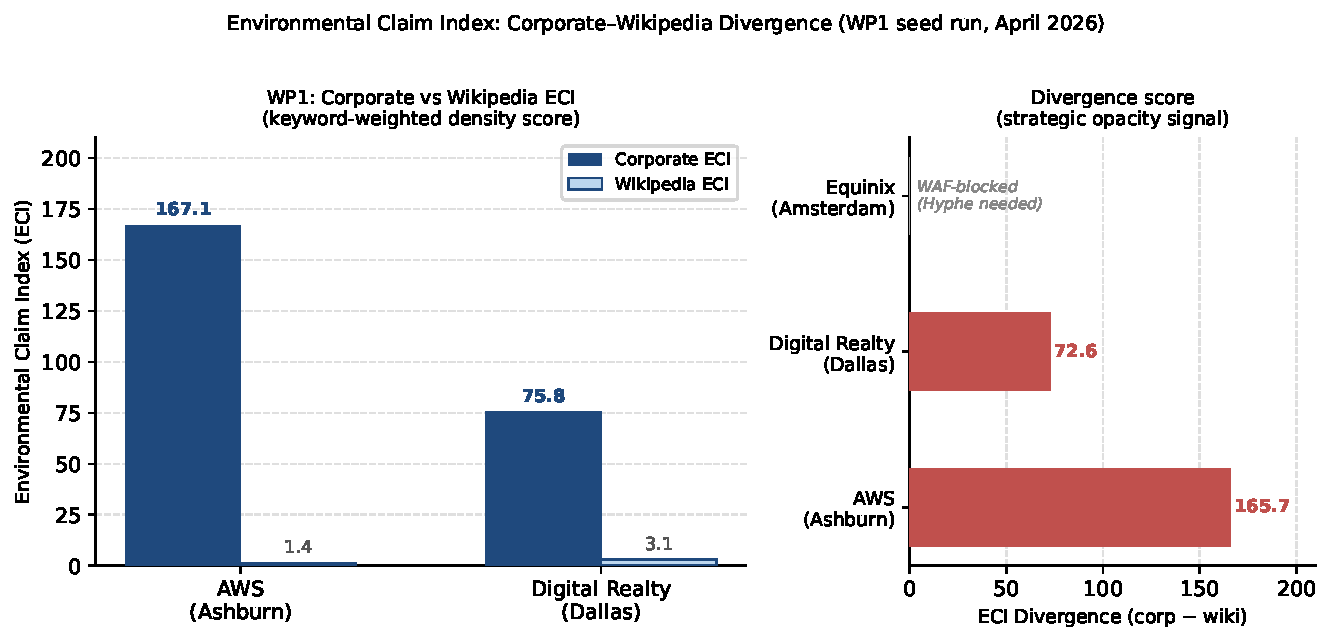
\includegraphics[width=\linewidth]{figures/wp1_eci_divergence}
\vspace{0.4em}
\captionof{figure}{WP1 seed results: Environmental Claim Index (ECI) for corporate websites versus Wikipedia articles (left), and ECI divergence gap per operator (right). A high divergence score indicates an operator constructing environmental claims that are decoupled from territorial accountability. Equinix's corporate site was blocked by a WAF, itself a finding. Data: pipeline run, April 2026.}
\label{fig:eci_divergence}
\end{fullwidth}

\subsection{WP2: Visual and Strategic Invisibility}

Data centers are designed, at considerable expense, to look like nothing. The suppression of windows, signage, and human scale is not an incidental feature of industrial economy but a deliberate act of visual engineering. WP2 treats this designed invisibility as a constitutive element of the assemblage rather than a communications strategy layered onto it: what operators choose not to show is as analytically significant as what they do show.

The work package operates across two parallel streams of visual material. The first is Sentinel-2 satellite imagery acquired at 10-metre resolution for a 500-metre bounding box around each facility coordinate — a state-derived, operator-independent account of the physical footprint that records building envelopes, cooling infrastructure, car parks, and spatial relationships to adjacent land uses that operators do not control and cannot redact. The second stream is corporate-published imagery scraped from operator websites: sustainability pages, facilities pages, and about-us sections, collected with full respect for robots.txt and assembled into per-operator manifests that record image files, alt text, and surrounding page context.

The analytical pipeline extracts Pillow-based visual metrics from each image — dimensions, aspect ratio, dominant colour — and assigns a content category: \textit{abstract} (server rooms, racks, logos, sustainability iconography), \textit{exterior} (building facades, campuses, cooling towers), or \textit{unknown}. Classification draws on alt text keyword matching as a baseline, with optional zero-shot CLIP or ResNet50 classification. From these labels a scalar \textit{visual abstraction score} — the ratio of abstract to total labelled images per operator — is computed. This score operationalises the degree to which an operator's visual self-presentation is decoupled from the material specificity of its facilities.

The abstraction score is not merely a measure of communications strategy. It is a governance claim. Visual substitution of abstract, placeless imagery for exterior location shots performs the cloud imaginary at the moment planning authorities and communities are contesting that framing. A jurisdiction comparison — operationalised through a Kruskal-Wallis test across facilities grouped by disclosure regime — tests whether visual abstraction is systematically associated with lighter regulatory environments. The predicted pattern, grounded in the comparative case: high abstraction in Loudoun County, where disclosure requirements are low and hyperscale anonymity is the default; lower abstraction in Amsterdam, where Dutch planning law and public debate have created a higher-disclosure environment in which operators face pressure to account for their footprint.

A first empirical pass of the satellite pipeline against the three seed facilities (April 2026) has yielded three analytical layers. Sentinel-2 RGB imagery at 10-metre resolution provides the baseline exterior record. Landsat 8/9 Land Surface Temperature (LST) composites for summer 2024 — derived from the ST\_B10 thermal band, converted to degrees Celsius at 30-metre resolution, across a 3\,km bounding box — make the thermal footprint of each facility visible as a heat signature: the consequence of round-the-clock cooling operations that operators do not publish and that no corporate image catalogue contains. VIIRS nighttime lights annual composites (NOAA DNB monthly V1, 2014--2024, 500-metre resolution, 10\,km radius) provide a longitudinal electricity-intensity record that is independent of operator disclosure.

The VIIRS time series produces a structurally revealing pattern. Ashburn shows a net increase in mean radiance of $+8.7\%$ between 2014 and 2024 --- the only jurisdiction in the seed sample with net positive growth (\Cref{fig:nightlights_ts}). Amsterdam records a $-9.2\%$ decrease over the same period, attributable to city-wide LED street lighting transition rather than reduced data center activity --- a measurement confound that is itself analytically instructive: in dense urban environments, the nighttime light proxy is attenuated by competing illumination sources and technology transitions, making the exurban Ashburn context the cleaner measurement environment. Dublin is flat at $-1.6\%$. The pattern is consistent with the WP3 land-use finding: deliberate spatial separation of the Ashburn cluster from residential settlement creates not only a governance gap but a cleaner physical signal.

The LST maps (\Cref{fig:lst_map}) make the thermal body of the assemblage visible at the site level. Cooling towers and server exhaust produce identifiable heat plumes extending beyond the facility perimeter — physical evidence of the energy flows that the cloud imaginary renders placeless. The contrast between the thermal profile of the Ashburn cluster --- an isolated heat source in an otherwise low-temperature exurban landscape --- and the Amsterdam facility --- whose thermal signature blends into the urban heat island, making it less legible as a discrete actor --- mirrors the governance contrast: physical embeddedness shapes the conditions under which communities can identify, attribute, and contest the infrastructure's impacts.

\begin{fullwidth}
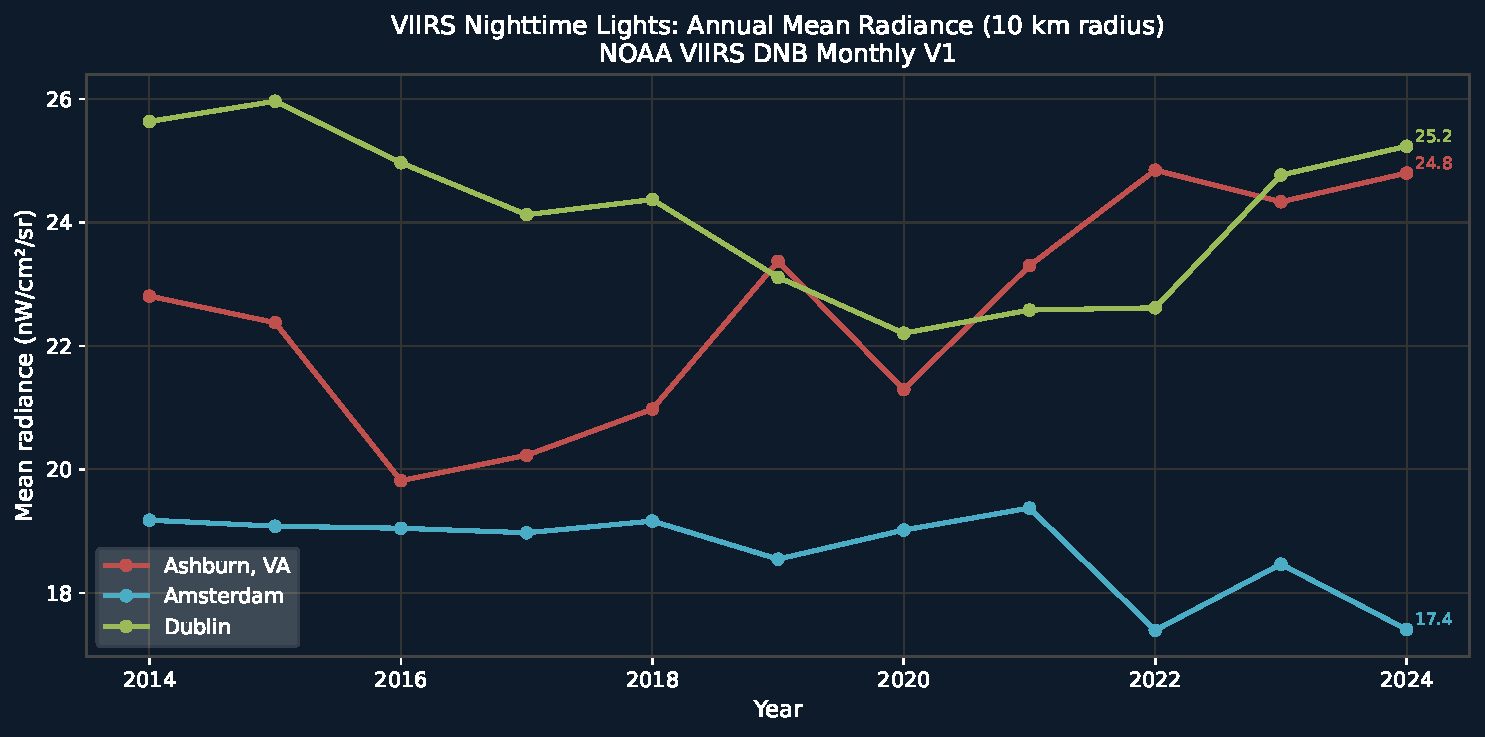
\includegraphics[width=\linewidth]{figures/wp2_nightlights_timeseries}
\vspace{0.4em}
\captionof{figure}{VIIRS nighttime lights: annual mean radiance (nW/cm\textsuperscript{2}/sr) within a 10\,km radius of each seed facility, 2014--2024 (NOAA VIIRS DNB Monthly V1, 500\,m resolution, Google Earth Engine). Ashburn is the only jurisdiction with net radiance growth ($+8.7\%$), consistent with data center cluster expansion in a low-background exurban context. Amsterdam's decrease ($-9.2\%$) reflects LED street lighting transition, a measurement confound that is more severe in dense urban environments. Data: GEE pipeline run, April 2026.}
\label{fig:nightlights_ts}
\end{fullwidth}

\begin{fullwidth}
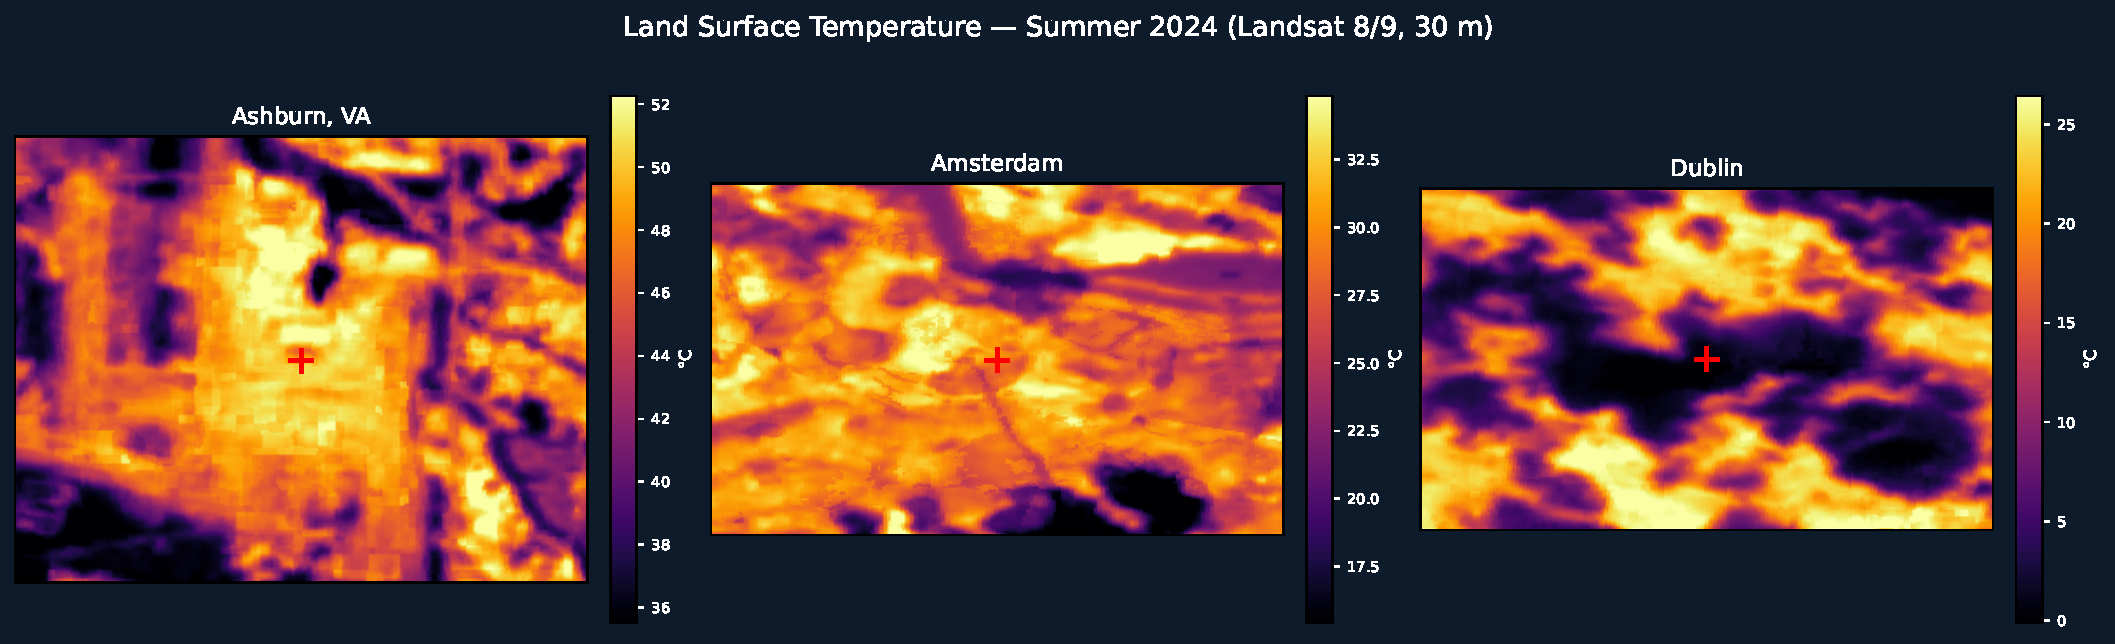
\includegraphics[width=\linewidth]{figures/wp2_lst_map}
\vspace{0.4em}
\captionof{figure}{Land Surface Temperature (LST) maps for the three seed facilities, summer 2024 composite (Landsat 8/9 Collection 2 Level-2, ST\_B10 band, June--August, $\leq 20\%$ cloud cover, 30\,m resolution, 3\,km bounding box). Red crosshairs mark facility centroids. The Ashburn facility sits within a discrete heat plume isolated from the surrounding low-temperature exurban landscape; Amsterdam and Dublin thermal signatures are embedded in the urban heat island. Data: GEE pipeline run, April 2026.}
\label{fig:lst_map}
\end{fullwidth}

The satellite record is, in this sense, the second measurement of the same gap that WP1 identifies in the textual record. Where WP1 finds a corporate ECI more than 120 times the Wikipedia score for Ashburn, WP2 finds a growing heat scar in the Virginia landscape that no corporate image catalogue contains. The operator narrates sustainability; the satellite records the thermal consequence of round-the-clock cooling. These are not independent findings that happen to be consistent: they are two modalities reaching the same sociotechnical fact --- the deliberate production of invisibility in one register does not alter the physical signature detectable in another. The divergence between what is claimed (clean, weightless, renewable infrastructure) and what is visible (an isolated, energy-intensive, thermally anomalous cluster) is the central analytical object of this work package, and it is only accessible through the juxtaposition of modalities that neither the textual nor the satellite record can achieve alone.

The four work packages and their mapping to CAS dimensions are summarised in \Cref{tab:wps}. Together, WP1 and WP2 map the conceptual dimension of the assemblage: the imaginaries through which data center infrastructure is made visible or invisible, the textual and visual acts through which territorial accountability is produced or evaded, and the variation in these across governance regimes that the CAS framing predicts will produce different structural and temporal outcomes.

%% Section 4 — Structural Dimensions
\section{Structural Dimensions: Ownership, Actor Constellations, and Urban Embeddedness}
\label{sec:structural}

The structural dimension of a CAS, in the Phillips and Ritala (2019) framework, concerns the hierarchy, relationships, and actor constellations that constitute the system's observable architecture. For data center assemblages, this is the dimension that the technical efficiency literature most systematically ignores and that the existing socio-political literature reaches only qualitatively. Who actually owns this infrastructure, in what legal form, and with what consequences for governance? Which actors are constitutive of the assemblage, and through what relationships do they interact? How is the infrastructure embedded in the urban and territorial systems through which it is contested, permitted, and supplied? Work Package 3 addresses the financial and ownership architecture; the city2graph framework \citep{city2graph} provides the tools for the urban-embeddedness layer.

\subsection{WP3: Ownership Cartography and Financialisation}

The question of ownership is not peripheral to the governance dynamics of data center assemblages — it is structural. The dominant ownership form in the world's largest data center market, Northern Virginia's Loudoun County, is the Real Estate Investment Trust. Equinix, Digital Realty, Iron Mountain, and a set of non-traded private REITs collectively control the majority of leasable capacity in the region. The REIT structure is not merely a tax-efficiency mechanism; it is a governance-relevant legal form with direct implications for accountability.

By distributing beneficial ownership across retail investors, pension funds, and sovereign wealth funds, the REIT dissolves the concentrated accountability that would otherwise attach to a single identifiable owner. No single shareholder holds a position large enough to bear reputational or political pressure from local contestation. More consequentially, the operating entity — the colocation provider or tenant REIT — is legally distinct from the asset-owning entity, which is in turn only one fund within a diversified investment vehicle whose beneficiaries are spatially dispersed and, in aggregate, politically inert. When community campaigns, planning bodies, or municipal authorities seek a counterparty capable of making binding commitments about energy sourcing, water use, or capacity limits, the REIT structure provides no such counterparty. The governance surface area — the interface at which political pressure can produce accountable response — has been systematically reduced by a legal form whose primary design purpose is unrelated to planning.

This condition, which we term the \textit{financialisation of digital infrastructure}, is mapped through a pipeline that resolves operator and owner company names from the project's facility index against the OpenCorporates company registry API. For each entity, the pipeline retrieves canonical legal identities, jurisdiction codes, incorporation dates, company type designations, and registered officer networks — a corporate-registry layer that is a prerequisite for the ownership graph, since operating company names frequently diverge from registered names, and holding structures often pass through multiple jurisdictions before reaching an identifiable beneficial owner. The pipeline's output — an auditable trail from facility-index name to registered corporate identity — feeds a network construction step that joins OpenCorporates records, officer data, and REIT asset schedules into a unified ownership graph.

The analytical products of WP3 are two. The first is an \textit{ownership network} in which nodes are legal entities — facilities, operating companies, holding companies, investment funds, and ultimate beneficial owners — and edges are ownership, directorship, and investment relationships. The second is an \textit{actor typology} that distinguishes between vertically integrated operator-owners, colocation operators leasing REIT-held assets, financial asset managers with no operational function, and public or quasi-public entities. These two outputs together constitute the structural map that WP3 contributes: a representation of the hierarchical and relational architecture of the assemblage that makes the governance consequences of ownership form legible.

\begin{figure}[ht]
\centering
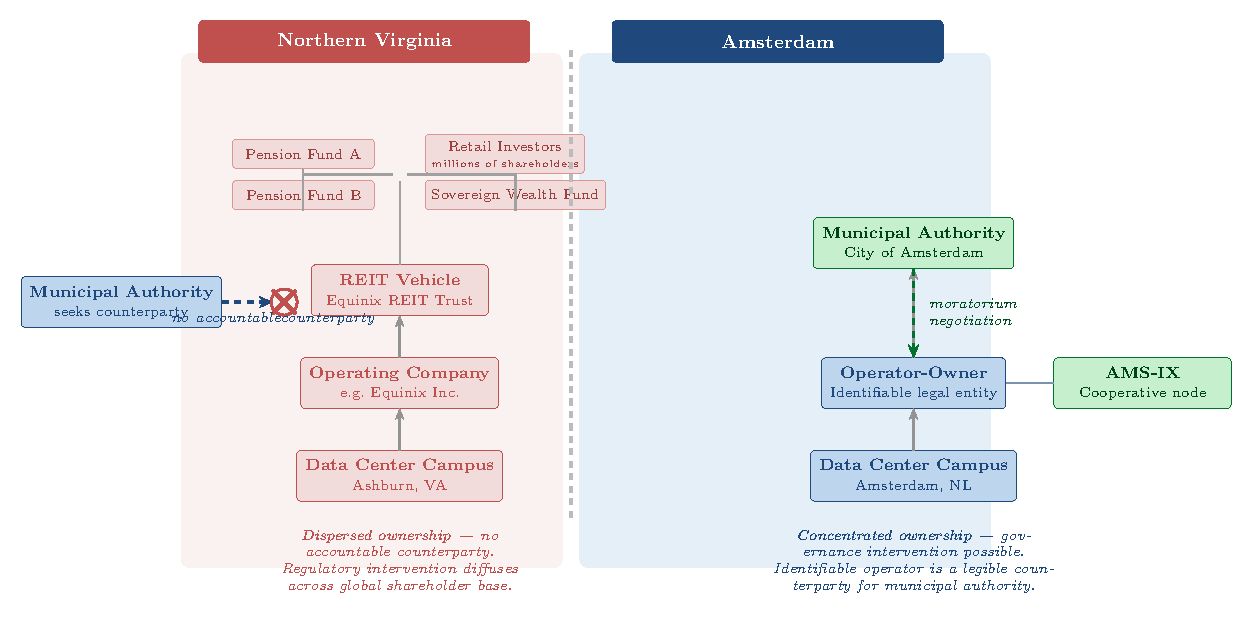
\includegraphics[width=0.92\textwidth]{figures/ownership-contrast}
\caption{Ownership structures and governance capacity: Northern Virginia (REIT-dominated, dispersed) versus Amsterdam (mixed, operator-owned, accountable). The structural difference explains the differential regime response to equivalent contestation intensity.}
\label{fig:ownership}
\end{figure}

The European ownership landscape is structurally different in ways that matter for regime response. Amsterdam's data center market, which experienced a formal moratorium between 2019 and 2022, exhibits a more varied ownership ecology: operator-owned campuses, a cooperative internet exchange (AMS-IX), and sovereign wealth fund investment that, unlike dispersed REIT ownership, is concentrated enough to constitute a visible and accountable actor in governance negotiations. The Netherlands' planning law structures accountability differently, creating clearer channels from municipal authority to identifiable ownership entities. This is not to argue that European ownership structures are uniformly more accountable — US-listed REITs are actively extending their European portfolios, and the structural conditions that make Virginia's governance gap possible are being reproduced in modified form across European markets — but rather that the structural composition of ownership shapes the surface area available for governance intervention in ways the CAS framing makes analytically tractable.

\subsection{Urban Embeddedness and Multi-Actor Constellations}

The ownership cartography of WP3 maps the financial architecture of the assemblage. But the assemblage's actor constellation extends considerably further: to the municipal governments that issue planning permissions, the energy utilities that negotiate grid connections, the water authorities that license abstraction, the residential communities that organise campaigns, the regional transport and land-use planners whose decisions shape what sites become available, and the civic institutions — schools, hospitals, industrial estates — that share the infrastructure on which data centers draw.

These actors are embedded in, and interact through, urban and territorial systems whose spatial structure shapes the possibilities for contestation and governance. The city2graph framework \citep{city2graph} — which converts geospatial urban data into graph structures incorporating infrastructure networks, land use, mobility flows, and spatial proximity relationships — provides the technical basis for representing this embeddedness computationally. Applied to the facility index, city2graph enables the construction of a spatial-relational graph for each jurisdiction in which data center nodes are connected to the urban actors and infrastructure systems they draw on and affect: power grid nodes, water infrastructure, residential zones, transport networks, and the municipal institutions through which planning and governance authority is exercised.

This spatial-relational graph is not merely a background map. It is an analytical object that makes legible the properties of the assemblage that the CAS framing foregrounds: the heterogeneity of actors at multiple scales (from the data center campus to the regional grid to the continental fibre network), the spatial relationships through which contestation is organised (residential proximity, shared infrastructure, political constituency), and the structural differences between jurisdictions that produce different governance outcomes. The comparison of Northern Virginia's low-density exurban geography — in which the data center cluster is spatially separated from residential populations and politically dominant through its contribution to the Loudoun County tax base — with Amsterdam's dense urban-fabric embedding — in which facilities compete for the same land, water, and political attention as residential and cultural uses — is a structural comparison that the city2graph representation makes systematic rather than impressionistic.

A first empirical pass of the pipeline against the project's three seed facilities yields a structurally telling pattern. The script downloads Overture Maps infrastructure and land-use layers for a 2\,km bounding box and builds a heterogeneous graph connecting each facility node to proximate power substations, residential zones, and commercial zones. The Ashburn/AWS facility sits within reach of 36 power-infrastructure nodes --- substations, cables, transformers --- but registers only one residential zone within the 1\,km adjacency radius and zero adjacent-residential edges. The Amsterdam and Dublin facilities show the inverse: the former records 61 residential zones with 16 adjacency edges, the latter 361 zones with 61 edges. The Ashburn profile is not explained by data sparsity: Overture Maps coverage in Loudoun County is comprehensive. It reflects a land-use pattern in which the data center cluster and residential settlement are deliberately separated at the scale of the built environment --- a spatial enactment of the territorial imaginary that makes the infrastructure legible to industrial logistics but invisible to community life (\Cref{fig:urban_embed}).

\begin{figure}[ht]
\centering
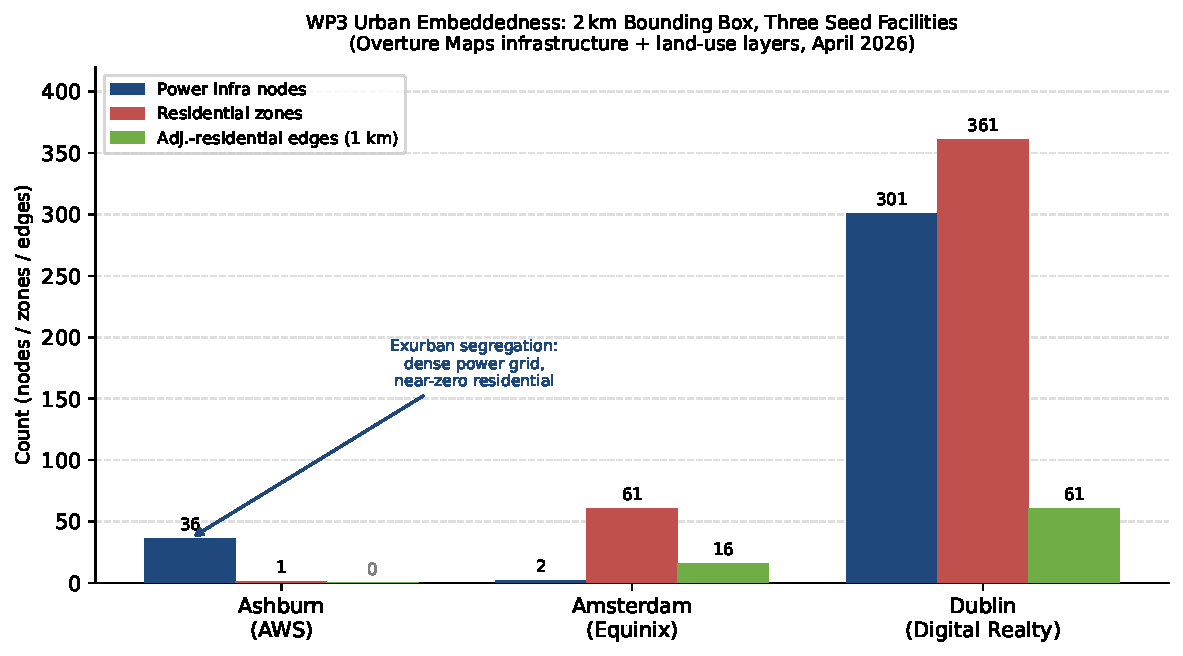
\includegraphics[width=0.90\textwidth]{figures/wp3_urban_embeddedness}
\caption{WP3 urban embeddedness results for three seed facilities (2\,km bounding box, Overture Maps infrastructure and land-use layers). Power infrastructure nodes (substations, cables, transformers), residential land-use zones, and adjacent-residential edges (within 1\,km) per facility. Ashburn's near-zero residential adjacency against its dense power infrastructure profile is a spatial signature of deliberate land-use segregation. Data: pipeline run, April 2026.}
\label{fig:urban_embed}
\end{figure}

\begin{figure}[ht]
\centering
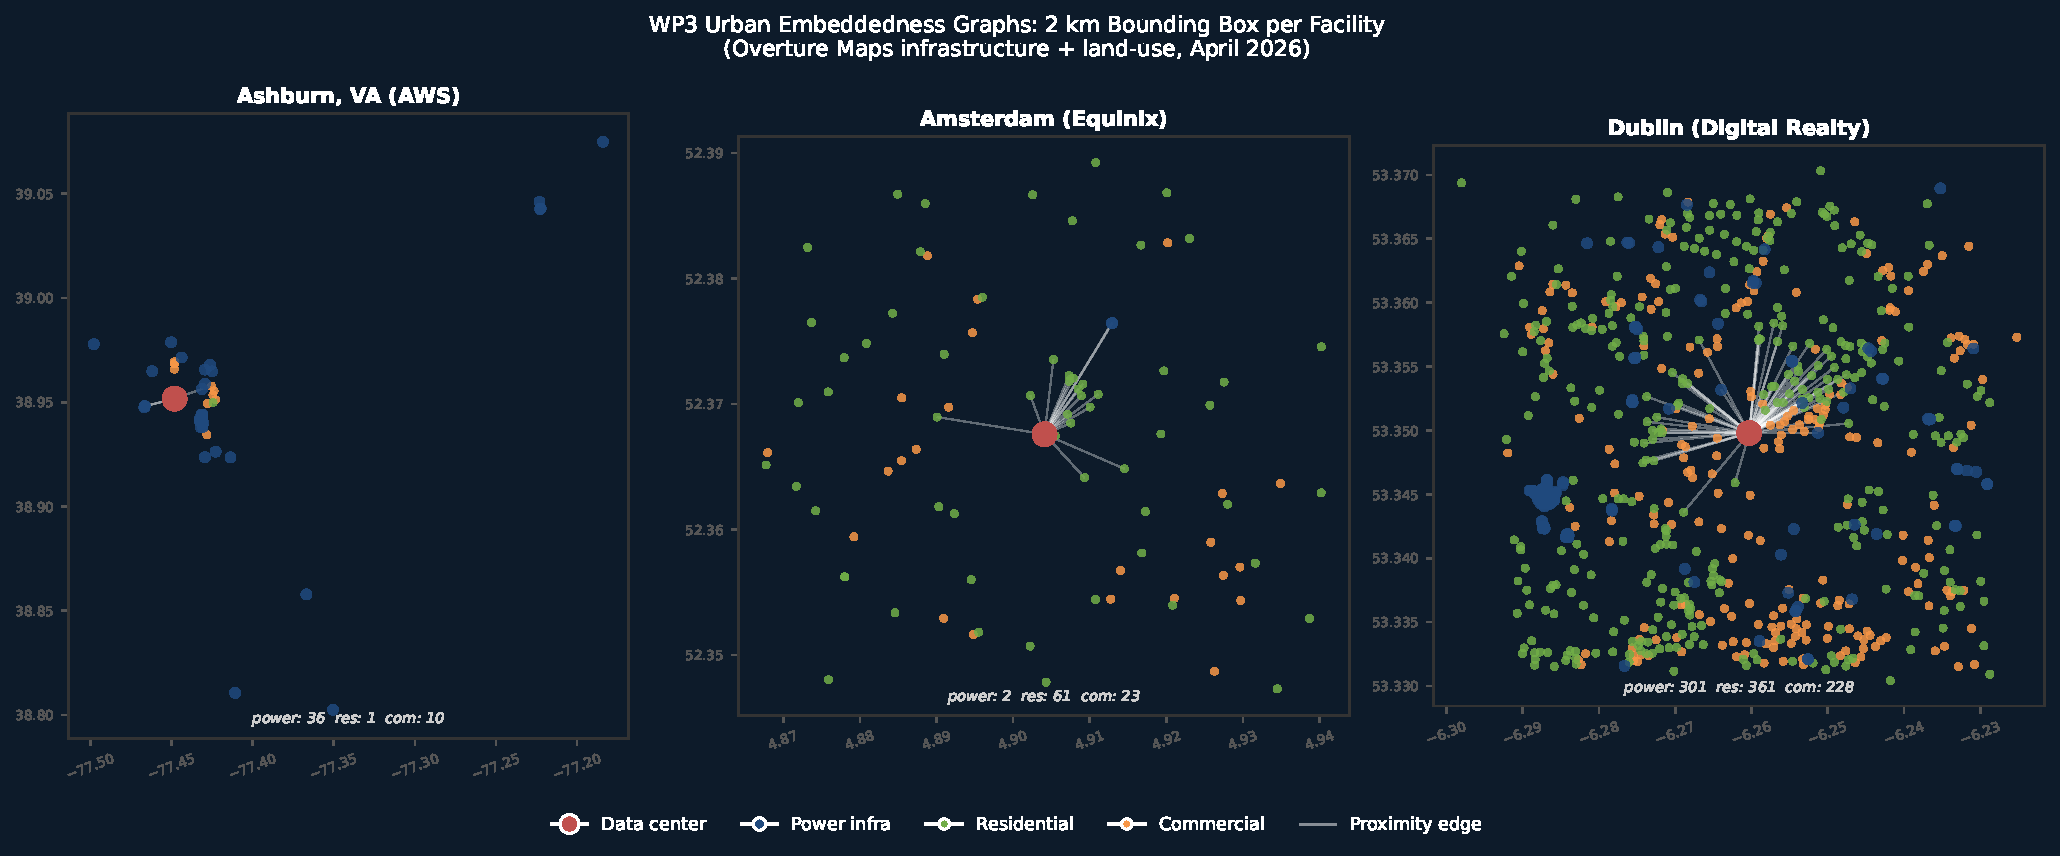
\includegraphics[width=\textwidth]{figures/wp3_urban_graphs_map}
\caption{Spatial urban graphs for the three seed facilities. Nodes are colour-coded by type: data center (red), power infrastructure (blue), residential zones (green), commercial zones (orange). Edges connect the data center to its $k$-nearest power nodes and to all residential zones within 1\,km. The visual contrast between the Ashburn graph --- a sparse residential-edge structure despite dense power connectivity --- and the Amsterdam and Dublin graphs is a spatial representation of the assemblage's embeddedness difference. Data: Overture Maps via city2graph, April 2026.}
\label{fig:urban_graphs_map}
\end{figure}

%% Section 5 — Temporal Dimensions
\section{Temporal Dimensions: Contestation Signals and Regime Response}
\label{sec:temporal}

The first three work packages produce largely synchronic portraits of the datacentering assemblage: how operators narrate themselves, how facilities are rendered visible or invisible, how ownership is constituted through financialisation. Each captures the system's structure at a point in time. The temporal dimension of the CAS, by contrast, concerns dynamics and co-evolution — how the system changes in response to disturbance, and under what structural conditions those changes constitute adaptation rather than absorption. Work Package 4 introduces time. Its purpose is to detect, track, and compare the arc of community contestation against data center development, from the first signs of organised opposition through to whatever regime response, if any, that opposition eventually produces.

\subsection{WP4: Contestation Signals}

The empirical core of WP4 is a multi-source contestation signal corpus assembled from three parallel data streams. News archives — regional and national press accessed via GDELT, NewsAPI, or MediaCloud — provide a longitudinal record of how contestation enters public discourse, how it escalates, and how operators and regulatory actors respond in the textual public sphere. Planning records — council minutes, formal objection filings, environmental impact assessments, moratorium orders — supply the institutional trace of how public signal is translated into regulatory action, with the temporal granularity required to identify discrete transition points. Social media data — principally X/Twitter and Reddit community boards — captures faster-moving, lower-threshold mobilisation that typically precedes or accompanies formal planning processes and provides a signal of contestation intensity that is independent of its institutional reception.

The analytical pipeline applies topic modelling (BERTopic applied to the news and social media corpus) to surface the thematic clusters through which contestation is articulated — energy demand, noise pollution, water consumption, land use conflict, planning law, municipal authority — and tracks how these frames shift as the contestation episode evolves. Event detection algorithms identify discrete inflection points in the longitudinal record: first substantive press coverage, first formal planning objection, moratorium filing, regulatory decision. From these event markers, the pipeline computes the \textit{signal-to-response lag}: the elapsed time between measurable community mobilisation and identifiable regime action, or the absence of any such action at the end of the observation window. This lag variable is the primary comparative output.

The lag variable is WP4's core theoretical contribution to the CAS argument. Complex adaptive systems are characterised not only by their compositional structure — the hierarchies and relationships that WP3 maps — but by the dynamics of adaptation: how the system responds to disturbance signals generated by its components. Community contestation is precisely such a disturbance, and the signal-to-response lag operationalises the key empirical question: under what structural conditions does community feedback produce adaptive regime response? Read alongside WP3's ownership cartography — which establishes how regulatory accountability is distributed or dissolved across ownership tiers — the lag variable becomes a structural diagnostic: it reveals whether a given assemblage configuration is capable of translating local resistance into systemic adjustment, or whether the structural properties of the system (dispersed ownership, legally separated operating and asset-holding entities, fragmented planning authority) insulate it from the disturbances its components generate.

The comparative design makes this concrete. Amsterdam declared a moratorium on new data center construction in 2019, enforced a development halt across the metropolitan region, and lifted the moratorium in 2022 under a differentiated framework requiring stringent energy-efficiency and water-use criteria — a full transition episode with identifiable onset, negotiation, and resolution. Northern Virginia presents the structural contrast: comparable contestation intensity over the same period, no moratorium, and an operator-accommodating state permitting environment that dispersed local accountability rather than consolidating it. The variable that differs is not signal strength but regime structure. The Amsterdam system, as WP3 establishes, had identifiable governance counterparties, concentrated ownership positions capable of entering into binding commitments, and a municipal planning authority with the legal competence to act. The Northern Virginia system, structurally constituted by dispersed REIT ownership, had no equivalent counterparty. WP4 makes this contrast measurable: the same community signal produces different trajectories in the two systems, and the lag variable captures the difference empirically.

As of April 2026, a seed contestation corpus has been constructed from the documented public record — drawing on academic sources \citep{vonderau2019storing}, regional and national press (the \textit{Washington Post}, \textit{Loudoun Now}, \textit{Irish Times}, \textit{The Oregonian}), and official regulatory documents (EirGrid grid capacity reports, Amsterdam Municipality planning decisions, An Bord Pleanála rulings) — across four jurisdictions: Amsterdam, Ashburn/Northern Virginia, Dublin, and The Dalles (Oregon). The corpus documents 58 discrete events between 2007 and 2025, annotated with date, source, and tone valence (\Cref{fig:contestation_signal}). The full live GDELT pull, automated corpus construction, and BERTopic topic modelling are deferred to the server pipeline run; the seed corpus is a methodologically transparent placeholder that establishes the temporal structure of each case and supports the manual cross-case comparison.

The seed corpus supports three first-order observations. First, contestation signal onset differs systematically across jurisdictions: Amsterdam reaches threshold intensity (three or more negative-tone events in a year) in 2019, Dublin in 2020, and Ashburn in 2021. The Dalles, a water-conflict jurisdiction, shows a lower-frequency, episodic contestation pattern with no clear onset year under the threshold measure. Second, negative-tone events constitute the majority of coverage in all jurisdictions (Amsterdam 56\%, Ashburn 59\%, Dublin 81\%, The Dalles 56\%), with Dublin showing the highest sustained negativity — consistent with EirGrid's grid-capacity warnings and An Bord Pleanála's high refusal rate. Third, regime response differs sharply from signal strength: Amsterdam's moratorium (2019) follows signal onset by less than one year; Northern Virginia, with comparable cumulative signal by 2022, produces no moratorium, consistent with the WP3 structural finding that REIT-dominated ownership provides no governance counterparty.

The operationalisation of key constructs — which events constitute signal onset, which count as regime response, how to handle gradual regulatory transitions of the kind Amsterdam's 2022 resolution represents — requires conceptual specification before computation can begin. This is the work package to which the open research community can contribute most immediately: local knowledge about specific contestation episodes, access to municipal planning archives not available through automated collection, and linguistic expertise for non-English jurisdictions are all resources the distributed observatory model is designed to aggregate.

\begin{fullwidth}
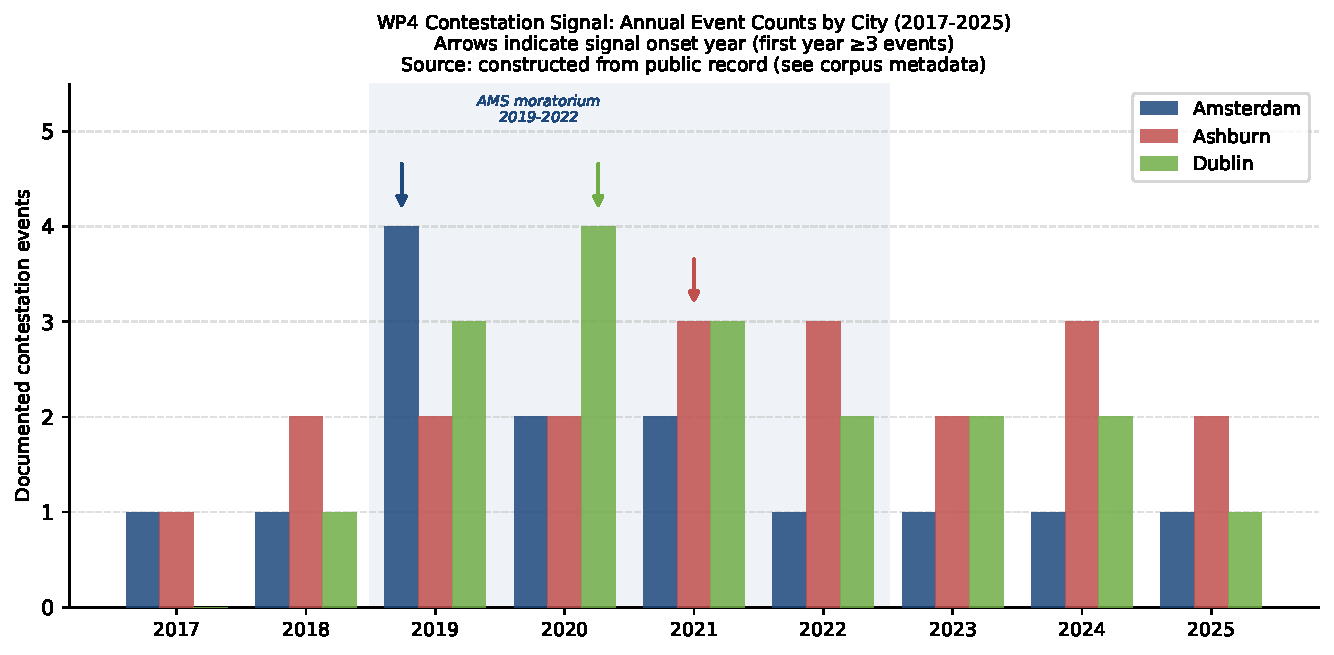
\includegraphics[width=\linewidth]{figures/wp4_contestation_signal}
\vspace{0.4em}
\captionof{figure}{WP4 seed contestation corpus: annual event counts by city (2017--2025), tone-coded. Shaded band: Amsterdam moratorium period (2019--2022). Onset arrows mark the first year reaching the threshold of $\geq 3$ events. Dublin's sustained high negative-tone volume reflects EirGrid grid-capacity constraints and An Bord Pleanála refusals; Northern Virginia's high volume without regime response is the structural contrast case. Data: seed corpus constructed from documented public record (58 events); full GDELT pull deferred to server run.}
\label{fig:contestation_signal}
\end{fullwidth}
%% Section 6 — Illustrative Case
\section{An Illustrative Comparison: Northern Virginia and Amsterdam}
\label{sec:case}

The following comparison is explicitly illustrative rather than causal. \Cref{tab:comparison} summarises the key dimensions across the two cases; the sections below develop each in turn. Its function is to demonstrate the analytical purchase of the CAS sensemaking framework: to show that the conceptual, structural, and temporal dimensions, examined together and across data modalities, generate an explanation for differential governance outcomes that existing single-method accounts cannot produce. The comparison draws on published sources, secondary reporting, and the preliminary outputs of the WP1--WP4 pipelines run against the project's seed facility index, and it acknowledges this as a limitation to be addressed as the research programme develops.

\subsection{Northern Virginia: The Governance Gap}

Loudoun County, Virginia — marketed, with some accuracy, as ``Data Center Alley'' — is the single largest concentration of data center capacity on earth. Hyperscale campuses operated by Amazon Web Services, Microsoft, Google, and Meta, combined with colocation facilities run by Equinix, Digital Realty, and CyrusOne, have made the county responsible for an estimated 70 per cent of the world's internet traffic at peak. The physical scale is extraordinary: hundreds of server halls, cooling towers visible from the Dulles Toll Road, diesel generator farms staged at the perimeter of campuses whose footprint exceeds many industrial estates.

The \textit{conceptual dimension} of the Northern Virginia assemblage is dominated by the cloud imaginary in its most refined form. Corporate websites for the major operators present the region in terms of network density, carrier diversity, hyperscale capacity, and sustainability commitments that foreground renewable energy sourcing. What is conspicuously absent from this textual register is any acknowledgement of the material friction that has begun to surface in planning hearings, water studies, and local electoral politics: communities in the western parts of the county objecting to the pace of rezoning, state legislators raising questions about water consumption from the Potomac River basin, and municipal planners struggling to translate the county's data center tax revenues into infrastructure capable of absorbing the load. The WP1 divergence analysis flags a high sustainability-to-community ratio and a high ECI gap relative to the Wikipedia register for Ashburn — the characteristic signature of territorial imaginary production operating under low disclosure pressure.

The \textit{structural dimension} is defined by REIT ownership. The majority of leasable data center capacity in Loudoun County is held by publicly traded REITs whose beneficial owners are pension funds, retail investors, and sovereign wealth funds distributed across multiple continents. The WP3 ownership graph for the region reveals a structure in which no single actor — not the operators, not the asset owners, not the investment managers — bears the concentrated accountability that governance intervention requires. The county's planning authority has legal powers over development approvals but no mechanisms to address the governance consequences of dispersed beneficial ownership. The result is a political economy in which the community contestation signal is real, persistent, and growing, but the institutional architecture for translating that signal into regime response is structurally absent. The city2graph urban embeddedness layer reinforces this reading at the spatial scale: the Ashburn facility records 36 power-infrastructure nodes within its 2\,km bounding box but only one residential zone and zero residential-adjacency edges within 1\,km --- a spatial segregation that insulates the assemblage from community entanglement at the built-environment level, not merely at the ownership level.

\subsection{Amsterdam: The Moratorium Episode}

Amsterdam's data center market achieved a global concentration second only to Northern Virginia before the municipality declared a moratorium on new hyperscale development in 2019, effective initially as a pause and then extended through 2022 before being selectively lifted under conditions. The moratorium is a documented governance episode: its triggers, its negotiation, and its resolution are on the record in planning documents, municipal council proceedings, and the ethnographic account of \citet{vonderau2019storing}. It constitutes, for the purposes of this paper, the kind of full transition episode — with identifiable signal, regime response, and outcome — that the CAS temporal dimension is designed to analyse.

The \textit{conceptual dimension} of the Amsterdam assemblage differs from Northern Virginia in ways that are legible in the textual and visual registers. Operators communicating about Amsterdam facilities cannot produce the cloud imaginary without engaging its territorial consequences: the Dutch public and political discourse around data center energy and water consumption, the AMS-IX cooperative that has made the city's internet exchange role a matter of civic identity, and the presence of academic and journalistic attention that has made the infrastructure visible in ways unusual for this sector. The WP1 ECI divergence for Amsterdam is lower than for Loudoun County — though, crucially, whether this reflects genuine territorial embeddedness or a more sophisticated rhetorical absorption of regulatory critique remains an open analytical question, one that the divergence scoring alone cannot resolve but that the close reading the keyword matrix enables can begin to address.

The \textit{structural dimension} is the decisive variable. Amsterdam's data center market in 2019 included a sufficient proportion of operator-owned and cooperative infrastructure — most critically, the AMS-IX member-owned exchange — to create identifiable, accountable counterparties for the municipality's governance intervention. The city's planning system had the legal authority to act; the ownership structure provided entities capable of entering into binding commitments; and the spatial embeddedness of facilities in a dense urban fabric meant that the political constituency for action was geographically concentrated and electorally significant. These are the structural conditions that made the moratorium achievable --- not the intensity of the contestation signal, which was comparable to Northern Virginia, but the architecture of the system receiving it. The urban embeddedness data corroborates: 61 residential zones within 2\,km and 16 within 1\,km proximity means that any governance intervention necessarily negotiates with a politically concentrated and spatially proximate constituency.

\subsection{What the Comparison Demonstrates}

The Virginia--Amsterdam comparison demonstrates, in miniature, the analytical programme of the paper. The same external pressure — community and political contestation of data center development — produces structurally different outcomes across two contexts. The variable that differs is not signal strength but the CAS properties of the receiving system: the ownership architecture (concentrated and accountable in Amsterdam, dispersed and insulated in Virginia), the planning authority's governance capacity (legally empowered and spatially concentrated in Amsterdam, constrained and revenue-dependent in Virginia), and the territorial imaginary (contested and partially negotiated in Amsterdam, dominant and entrenched in Virginia). These are the structural and conceptual dimensions of the assemblage, and they are only visible simultaneously — the ownership graph alone cannot explain why the municipality could act, the text analysis alone cannot explain why the ownership structure mattered.

This is the argument for multimodality: not that more data is better, but that different data modalities reach different dimensions of the assemblage, and that no single dimension is explanatorily self-sufficient.

%% Section 7 — Discussion
\section{Discussion}
\label{sec:discussion}

\subsection{Multimodality as theoretical necessity}

The paper's methodological argument — that studying datacentering requires combining text, image, financial, and temporal data streams — is sometimes read as a claim about comprehensiveness: more data modalities produce a fuller picture. The argument of this paper is different. Multimodality is not an empirical strategy for reducing gaps but a theoretical necessity following from the CAS structure of the phenomenon.

Each data modality addresses a dimension of the assemblage that the others structurally cannot reach. The corporate text corpus captures the imaginary production through which operators constitute their infrastructure as placeless and their practices as responsible — a communicative act that shapes what becomes legible as a planning problem. Satellite imagery captures the material footprint independently of operator disclosure, providing the state-derived account against which imaginary claims can be read. Financial and ownership data reach the legal and investment architecture through which accountability is distributed or dissolved — a dimension entirely invisible to both text and imagery. And contestation signal data captures the temporal dynamics through which community mobilisation unfolds, escalates, and either produces regime response or dissipates without one.

The opacity of data center infrastructure is not a data gap to be solved with more comprehensive collection. It is a sociotechnical fact: the deliberate, sustained construction of illegibility is itself a constitutive feature of the assemblage, produced through architectural choices, legal structures, communications strategies, and the ``cloud'' metaphor's ideological work. A firm that will not publish its water consumption can still be found in a REIT filing. A campus designed to be visually indistinguishable from a warehouse is still visible in a Sentinel-2 image. A planning moratorium leaves traces in municipal council records even when operators prefer it unexamined. Multimodality is the methodological response to deliberate opacity: triangulation around the assemblage, not penetration of it.

\subsection{The open exchange as theoretically motivated design}

The most consequential implication of the CAS framing for research design is the one most likely to be read as peripheral to the scholarly contribution: the open research infrastructure. The argument of this paper is that the open exchange is not a nice-to-have or an act of scholarly generosity, but a theoretically motivated design choice that follows from the properties of the phenomenon.

Data center assemblages span hundreds of jurisdictions, thousands of facilities, multiple layers of ownership obscured by deliberate legal complexity, and contestation dynamics unfolding across years and decades. The knowledge required to map this — local expertise about specific planning disputes, access to national company registries, linguistic capacity across the jurisdictions involved, methodological knowledge across NLP, computer vision, network analysis, and event detection — is distributed across researchers, civil society organisations, journalists, activists, and community members in ways that no single research team can replicate. A CAS-like phenomenon of this scale requires a distributed observational infrastructure to match.

The research commons — the community-maintained facility index, the shared analytical pipelines, and the open data — is the governance architecture of a distributed observatory. The contributing guide that accompanies this paper is not supplementary documentation; it is part of the methodological argument, specifying the protocols through which distributed knowledge can be aggregated, quality-controlled, and made analytically tractable. When the bibliography of this paper includes a contribution from a local planner in Ashburn who submitted a facility record, or a journalist in Singapore who documented an unreported data center campus, the knowledge produced will be qualitatively different from what any single research team could produce — not just broader, but differently constituted, with a different relationship to the phenomena it describes.

This is the sense in which the open exchange is theoretically necessary: not because collaboration is virtuous, but because the CAS structure of the object demands a research architecture capable of matching its scale, distribution, and deliberate opacity.

\subsection{Positioning within innovation studies}

The paper's argument, if accepted, has implications for the broader innovation studies research programme that extend beyond the specific empirical domain of data centers.

The first implication concerns the object. Data center infrastructure is not a niche concern for digital geographers or infrastructure studies specialists. It is a transition-critical technology: the material substrate through which energy transitions, platform governance, digital sovereignty, and the greening of the economy are being simultaneously negotiated. An electricity consumer of 400~TWh annually that is growing at double-digit rates cannot remain outside the sustainability transitions research programme without that programme sustaining a significant blind spot in its understanding of the socio-technical regime within which energy transitions are occurring.

The second implication concerns the concept. ``Datacentering'' as a gerund is a methodological invitation as much as a theoretical claim. It asks researchers to shift their attention from the stable properties of a technology to the ongoing, contested, processual work of assembling, reproducing, and resisting it. This shift — from noun to gerund, from object to process — is the move that makes the MLP's distinction between landscape, regime, and niche applicable: the ``cloud'' regime is being assembled and contested in real time, and the contestation dynamics documented in this paper are the niche-level disruptions through which transition pressure is beginning to accumulate.

The third implication concerns the CAS framing itself. The risk of invoking complexity theory is that it becomes a theoretical free pass — a way of gesturing at systemic properties without specifying what they are or how they would be detected. The Phillips and Ritala (2019) three-dimensional structure disciplines this application: by committing to the conceptual, structural, and temporal dimensions as distinct but interrelated analytical targets, the paper specifies what an adequate account of the assemblage must reach, and it provides the methodological apparatus to reach each dimension. This is the sense in which the CAS lens functions as sensemaking rather than metaphor: it organises the research design without overclaiming about the formal properties of the system under study.

%% Section 8 — Conclusion
\section{Conclusion}
\label{sec:conclusion}

This paper began from a bibliometric fact: nearly five thousand publications on data centers, and not one engaging the theoretical frameworks through which innovation scholars analyse infrastructure transitions. The argument it has developed is that this gap is not incidental but produced — by a metaphor that naturalises the infrastructure, by a disciplinary division of labour that assigns it to engineers and ethnographers, and by the deliberate opacity that operators have constructed around it. The cloud conceals.

The concept of \textit{datacentering} is proposed as a remedy. The shift from noun to gerund is a shift in what we attend to: from the stable properties of a technology to the active, contested, ongoing process of assembling it. When we study datacentering rather than data centers, we immediately encounter the features that innovation scholars are trained to analyse — actors, governance, contestation, imaginaries, regime dynamics — and we immediately face the methodological challenge that those features present: they are constituted across multiple registers (textual, visual, financial, temporal), distributed across multiple scales (facility, city, jurisdiction, global network), and partially hidden by design.

The Complex Adaptive Systems framing, drawn from \citet{phillips2019complex} as a sensemaking lens rather than a formal model, organises the methodological response. The conceptual dimension of the assemblage — how actors construct imaginaries and manage visibility — is addressed through corporate and territorial text analysis (WP1) and visual and satellite imagery (WP2). The structural dimension — the ownership hierarchy and actor constellation through which governance capacity is constituted or dissolved — is addressed through ownership cartography (WP3) and urban-embeddedness analysis. The temporal dimension — how contestation unfolds and what determines whether regime actors respond — is addressed through contestation signal detection (WP4). Together, the four work packages constitute a multimodal cartographic methodology that is adequate to the CAS-like complexity of the object, and the Virginia--Amsterdam comparison demonstrates, illustratively, the analytical purchase of applying it.

The conclusion the paper reaches is that no single researcher or team can build this cartography alone. The geography is too large, the data too distributed, the opacity too deliberate, and the jurisdictional knowledge too local for any single team to map it adequately. This is not a counsel of humility but a methodological finding: the research commons is the only architecture adequate to the object's actual complexity. The open facility index, the shared analytical pipelines, the contributing protocols, and the GitHub Discussions are not supplementary to the scholarly contribution — they are part of it.

We therefore close with an explicit invitation. If you have local knowledge about a planning dispute, a facility that does not appear in published records, a moratorium under negotiation, or a community campaign in its early stages — that knowledge is analytically valuable and there is a structured place for it in this research infrastructure. If you have methodological expertise in NLP, computer vision, network analysis, or event detection — the pipelines are open and documented. If you have access to national company registries, REIT filings, or energy and water disclosure records that are not publicly accessible through the channels the project currently uses — get in touch.

The cloud is not a metaphor. It is infrastructure. And infrastructure, with the right tools and the right collaborators, can be mapped.


\bibliography{references}

\end{document}
